\chapter{L'analisi dei rischi}
La valutazione dei rischi rappresenta il momento fondamentale per la prevenzione delle criticit� nelle aziende con lo scopo di individuare e risolvere i problemi che � possibile riscontrare.
Esistono molti strumenti e tecniche disponibili per l'identificazione di potenziali pericoli e problemi di operabilit�, di seguito sono riportate i pi� utilizzati:
\begin{itemize}
	\item \textbf{Checklists}: lista di voci che occorre controllare e spuntare per verificare che una determinata serie di operazioni sia stata eseguita correttamente;
	\item \textbf{Fault Modes and Effects Analysis (FMEA)}: analisi eseguita preventivamente e quindi basata su considerazioni teoriche e non sperimentali. Come primo passo viene effettuata la scomposizione del sistema in sottosistemi, per ognuno di essi devono essere elencati tutti i possibili guasti e successivamente le cause e le conseguenze; \cite{uno}
	\item \textbf{Fault Tree Analysis}: tecnica analitica in cui innanzitutto viene individuato uno stato indesiderato in cui pu� venire a trovarsi il sistema e in seguito viene effettuata un'analisi per determinare tutti i modi credibili in cui l'evento indesiderato pu� verificarsi. \cite{due}
	\item \textbf{Studio "What-if"}: viene condotto utilizzando un approccio del tipo brainstorming; si inizia con l'analizzare pericoli gi� noti al team di lavoro per arrivare ad altri potenziali scenari incidentali;
	\item \textbf{HAZOP}: esercizio che si svolge attraverso la formulazione di alcune specifiche domande strutturate; � finalizzato all'individuazione di deviazioni dagli intenti di progetto che possono portare ad inconvenienti di sicurezza o di esercizio. \cite{tre}
\end{itemize}

Alcune tecniche, come le Checklists e lo Studio "What-If", possono essere utilizzate all'inizio del ciclo di vita del sistema o se non � richiesta un'analisi dettagliata; al contrario, se vogliamo avere informazioni pi� complete sui pericoli a cui � sottoposto il sistema � opportuno procedere con un'analisi HAZOP, tale tecnica verr� descritta e approfondita successivamente.\
\newline
Nella seguenti tesi verr� esposta l'hazard analysis dell'apparato IMR di RFI per la manutenzione delle varie linee ferroviarie.\\
L'obiettivo del lavoro � quello di individuare tutti i potenziali pericoli, sia quelli essenzialmente rilevanti per l'area immediata del sistema, sia quelli con una sfera di influenza pi� ampia.\\
Per effettuare tale lavoro � stata utilizzata la strategia \textbf{HAZOP} (	\textbf{HAZ}ard and \textbf{OP}erability analysis); tale tecnica ha avuto origine da studi di tipo assicurativo, specie su grandi impianti di processo, estendendo la sua applicazione ad ambiti e dimensioni diverse.
L'HAZOP mira all'individuazione dei pericoli esistenti nella gestione di un determinato processo lavorativo. Tali pericoli sono identificati e indagati sulla base di deviazioni, siano esse accidentali o meno, di parametri chiave, caratteristici del processo in esame. \cite{tre}\\
L'espressione \textit{analisi dei rischi} viene sinteticamente utilizzata per indicare un processo che in pratica comprende 4 fasi:
\begin{itemize}
	\item \textit{Definizione}: in questa fase gli obiettivi e lo scopo dell'analisi devono essere definiti. Questa prima fase � fondamentale per chiarire quali siano i confini del sistema e le sue interfacce con altri sistemi, in modo tale che l'analisi non si discosti in aree irrilevanti rispetto all'obiettivo;
	\item \textit{Preparazione}: questa fase ha lo scopo di ottenere le informazioni necessarie per effettuare l'analisi e di convertire tali informazioni in un formato adatto. In seguito deve essere riportata una descrizione del progetto contenente tutti i dettagli tecnici e amministrativi necessari. Devono essere fornite informazioni circa le condizioni ambientali in cui il sistema operer�, qualifiche, abilit� ed esperienza del personale operativo e di manutenzione e infine devono essere riportate le problematiche evidenziate in sistemi simili. Non di minore importanza � l'operazione di stima del tempo necessario per condurre l'analisi che deve essere eseguita in questo frangente; infine, devono essere scelte le parole guida pi� adeguate per condurre l'analisi del sistema, considerando che una parola guida troppo specifica pu� limitare le idee e la discussione, al contrario una troppo generica potrebbe non focalizzare lo studio in modo efficiente. Di seguito � riportata la lista delle parole guida:
	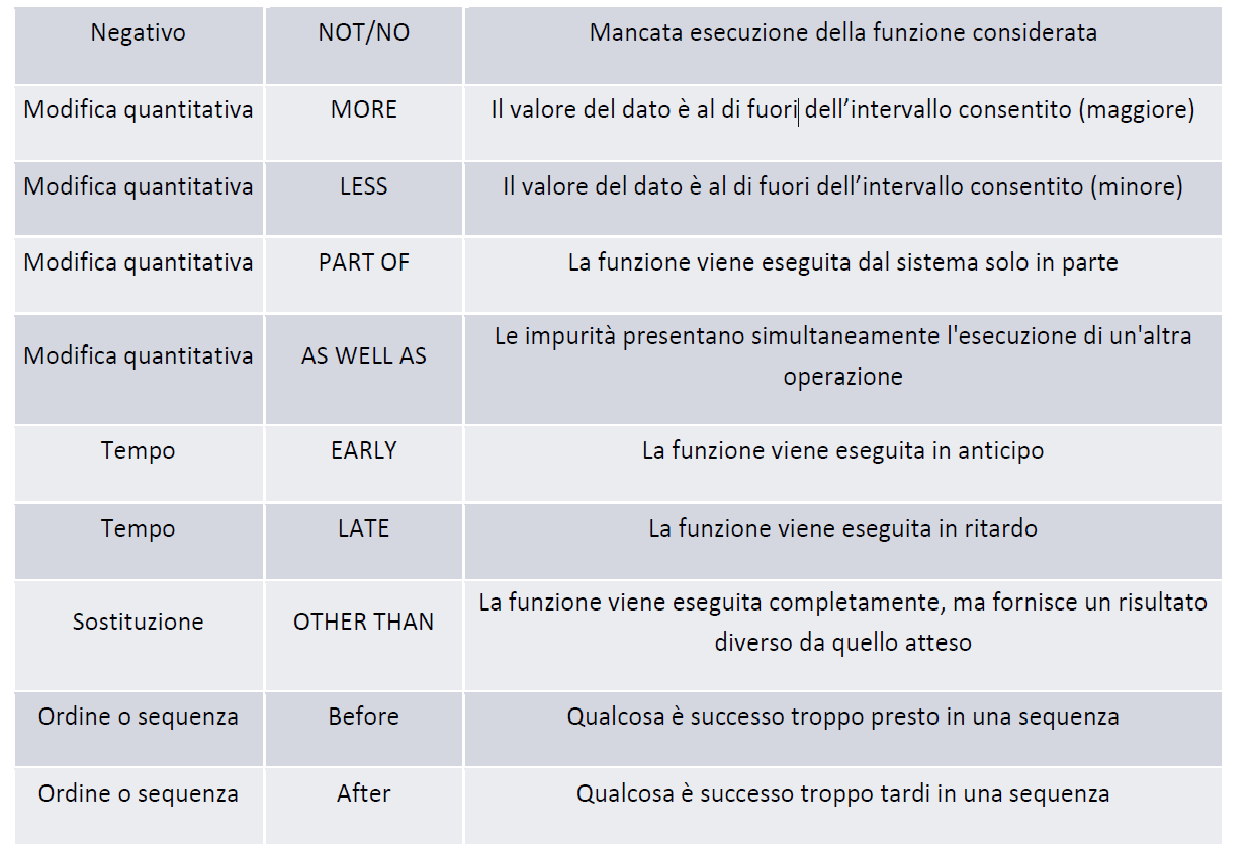
\includegraphics[scale = 0.5]{img/parolechiave}
	\item \textit{Esaminazione}: questa � la fase che rappresenta la vera e propria analisi del sistema. Come prima cosa viene diviso il sistema in parti, tale divisione deve essere effettuata in modo pertinente ai fini dell'analisi; in seguito deve essere spiegato il ruolo progettuale della parte in questione, gli elementi pertinenti e le eventuali caratteristiche associate agli elementi identificati.
	Per ogni parte del sistema devono essere individuate le parole guida appropriate, ovvero quelle che possono dar luce a eventuali criticit�. Le parole guida vengono esaminate nel contesto dell'elemento o della caratteristica studiata per rilevare eventuali deviazioni credibili dall'intento progettuale.\\ 
	Qualora venga trovata una deviazione credibile, viene effettuata un'indagine per individuare tutte le cause e le conseguenze. Le deviazioni vengono classificate in base al potenziale impatto e alla loro frequenza di accadimento, come vedremo in seguito. Di fondamentale importanza � identificare la presenza di meccanismi di protezione e rilevamento della deviazione che possono essere inclusi nella parte selezionata. Questo procedimento viene ripetuto per ogni parte del sistema, per ogni parola guida e per ogni sua interpretazione, al fine di riuscire a individuare tutti i rischi a cui il sistema pu� andare incontro.\\
	Quando una parte � stata del tutto esaminata, dovrebbe essere contrassegnata come completata. Di seguito viene riportato il diagramma di flusso della procedura appena descritta:\\
	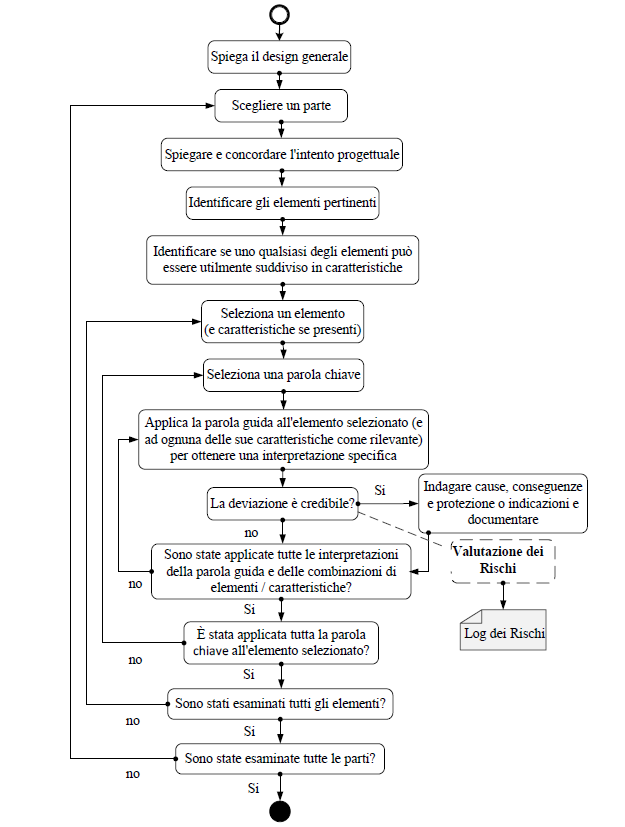
\includegraphics{img/diagrammaesame}
	\item \textit{Documentazione}: per completare l'analisi e ottenere tutti i suoi benefici � opportuno documentarla. Esistono due approcci per effettuare tale procedura: registrazione completa o solo per eccezione. La registrazione completa comporta la registrazione di tutti i risultati. Questo metodo pu� risultare ingombrante ma sicuramente completo di tutte le informazioni; al contrario, la registrazione delle eccezioni implica la memorizzazione esclusivamente dei rischi identificati e dei problemi di operabilit�. In tal caso la quantit� di dati da memorizzare � inferiore e sicuramente la gestione di questi ultimi � pi� semplice.\\ Una buona documentazione dovrebbe includere dettagliatamente quanto segue:
	\begin{itemize}
		\item dettagli dei pericoli identificati e problemi di operabilit�;
		\item raccomandazioni per eventuali ulteriori studi su aspetti specifici del progetto utilizzando tecniche diverse, se necessario;
		\item azioni necessarie per affrontare le problematiche individuate durante lo studio;
		\item un elenco di tutte le parti considerate nell'analisi, insieme alla motivazione associata all'eventuale esclusione di determinate parti del sistema;
		\item elenco di tutti i disegni, specifiche, schede tecniche, report, ecc...
	\end{itemize}
 Attraverso la registrazione per eccezioni le informazioni sui vari rischi sono descritte in maniera piuttosto concisa, senza riportare informazioni dettagliate.\\
 Nella documentazione ogni azzardo, problema operativo o pericolo, insieme alle proprie eventuali cause, dovrebbe essere registrato come elemento separato e indipendente.\\ Infine, dovrebbe essere adottato un sistema di numerazione per fare in modo che ogni rischio, problema operativo, mitigazione e raccomandazione venga identificato in maniera univoca. Per garantire il recupero della documentazione, � opportuno che essa venga archiviata.
\end{itemize}
 \subsection{Il processo per la valutazione del rischio}
 Come precedentemente anticipato nella fase di esaminazione � opportuno effettuare una valutazione del rischio riscontrato. \\
 \begin{figure}[htbp]
 	\centering
 	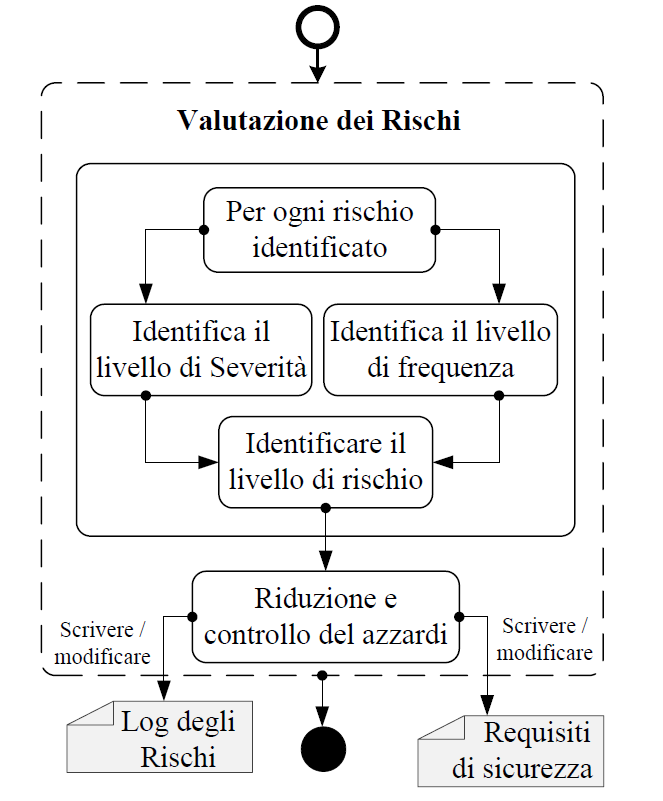
\includegraphics[scale=0.4]{img/valrischi}
 	\caption{Il processo per la valutazione dei rischi}
 \end{figure}
Le attivit� di valutazione del rischio vengono condotte con lo scopo di quantificare il rischio associato ad ogni pericolo. Per ogni comportamento anomalo individuato viene analizzata la frequenza di occorrenza e la sua severit�. Dal connubio di queste informazioni � possibile identificare il livello del rischio. 
\begin{figure}[htbp]
	\centering
	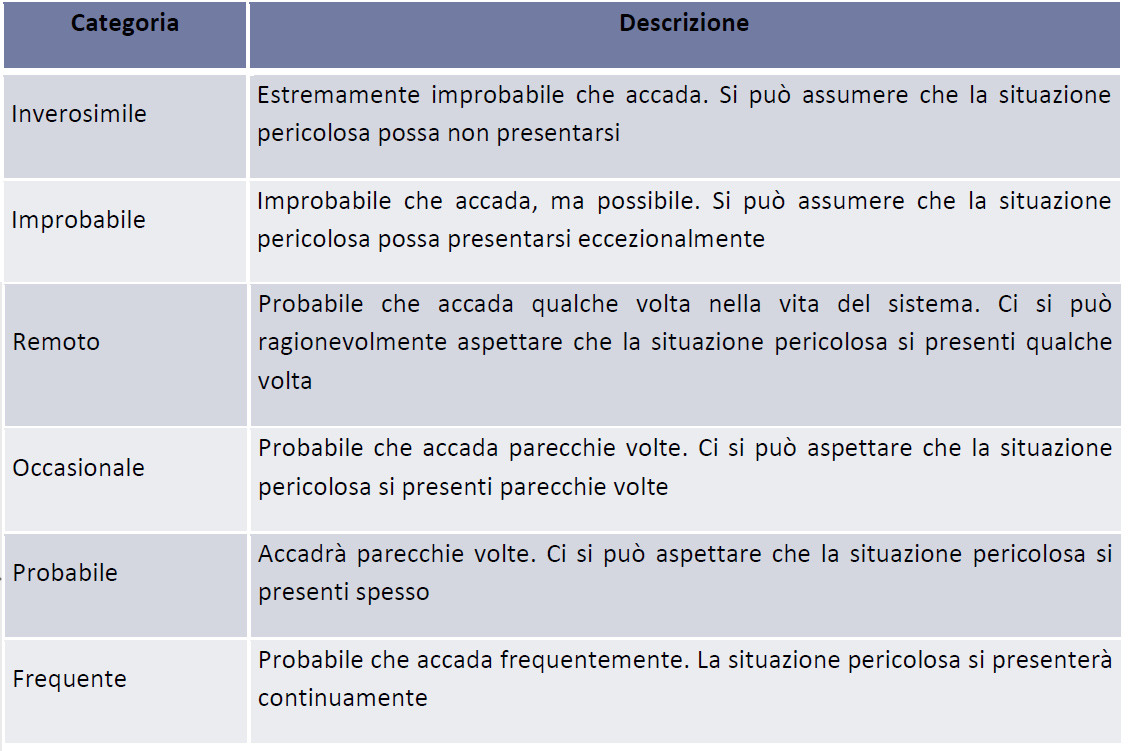
\includegraphics[scale=0.4]{img/frequenza}\\
	\caption{Tabella per la classificazione delle frequenze}
\end{figure}


\begin{figure}[htbp]
	\centering
	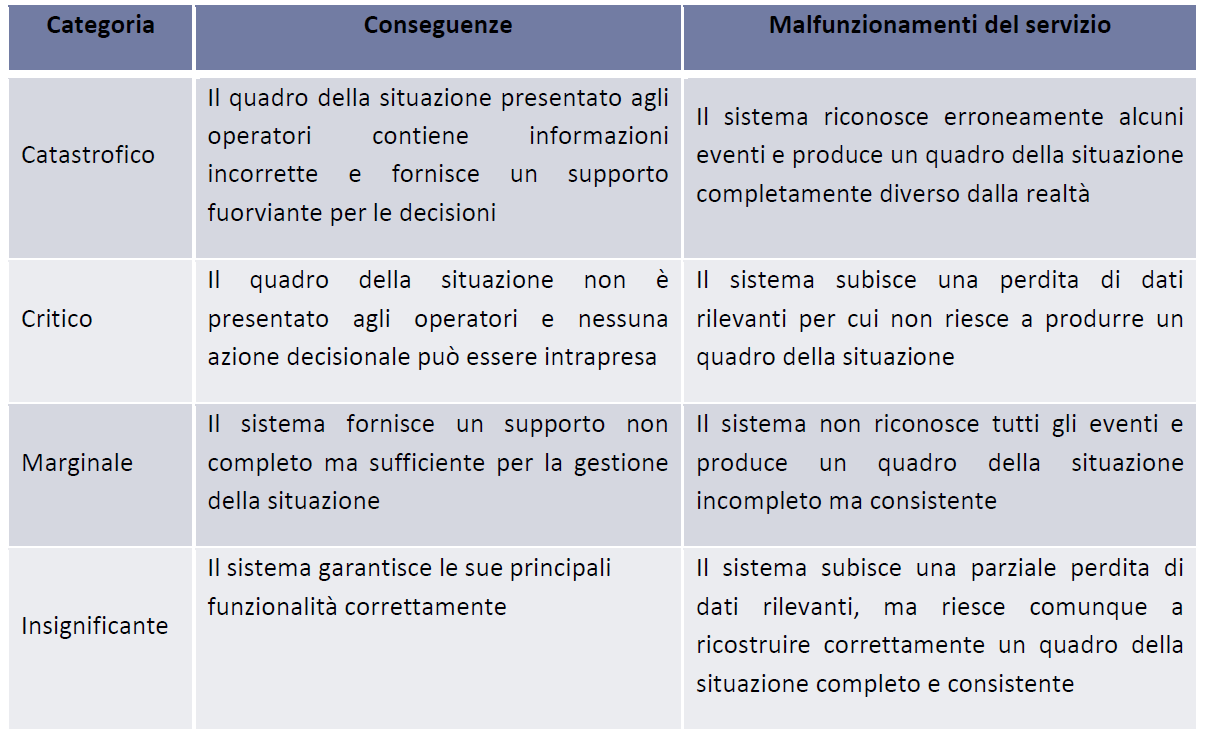
\includegraphics[scale=0.4]{img/severit}\\
	\caption{Tabella per la classificazione della severit�}
\end{figure}
Quest'ultimo pu� essere classificato come:
\begin{itemize}
	\item trascurabile
	\item tollerabile
	\item indesiderabile
	\item intollerabile.
\end{itemize} 
Qualora il livello del rischio sia trascurabile o tollerabile non � necessario individuare un'opportuna mitigazione, in quanto il verificarsi del rischio non viene ritenuto pericoloso nei confronti del sistema, ugualmente se l'incombensa del pericolo � altamente improbabile. Negli altri casi l'analisi procede con la ricerca dell'opportuna soluzione che avr� come scopo o ridurre la severit� del rischio oppure la sua frequenza di occorrenza.

	\begin{figure}[htbp]
		\centering
		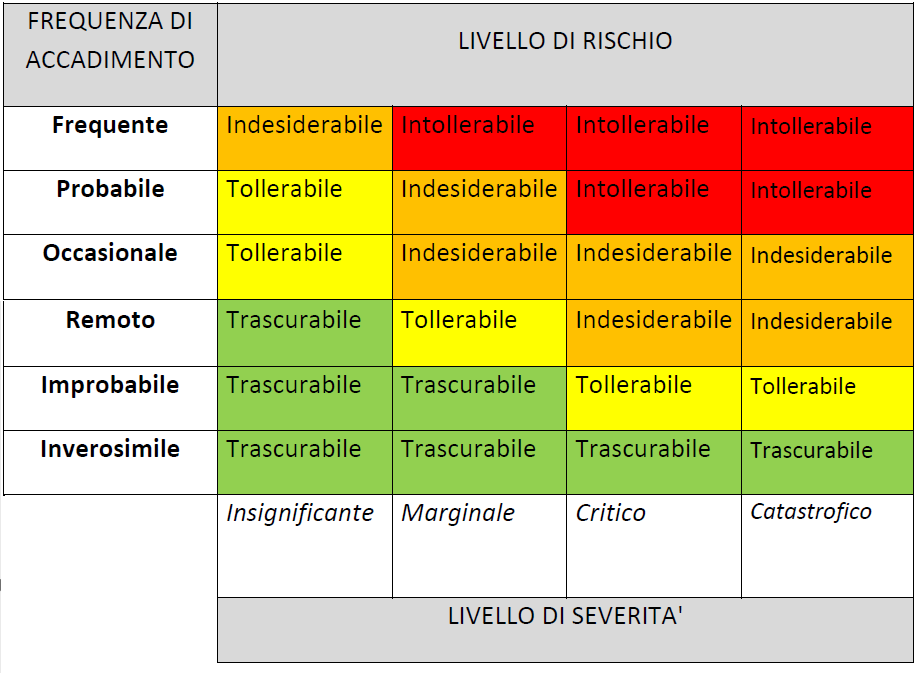
\includegraphics[scale=0.4]{img/risklevel}\\
		\caption{Risk Matrix}
	\end{figure}
	
 

